\documentclass{article}
\usepackage{tikz,amsmath,siunitx}
\usepackage{pgfplots}
\usepackage{listings}
\usetikzlibrary{arrows,snakes,backgrounds,patterns,matrix,shapes,fit,calc,shadows,plotmarks}
%\usepackage[graphics,tightpage,active]{preview}
%\PreviewEnvironment{tikzpicture}
%\PreviewEnvironment{equation}
%\PreviewEnvironment{equation*}
\title{CS540 Practice Assignment 8}
\author{Dustin Ingram, Aaron Rosenfeld, Tom Wambold}
\newlength{\imagewidth}
\newlength{\imagescale}
\pagestyle{empty}
\thispagestyle{empty}
\lstset{breaklines=true}
\begin{document}
\maketitle
\newpage
\section{Tasks}
\begin{enumerate}
    \item Implement and time a Parallel radix 2 divide and conquer WHT using Pthreads. Compute speedup compared to your sequential code. What was the smallest input size for which you obtained speedup?
    \item Implement and time parallel multiple WHTs, i.e. I\_M tensor W\_N using openMP.
    \item Implement and time a Parallel WHT, i.e. W\_MN = (W\_M tensor I\_N)(I\_M tensor W\_N), using OpenMP. Both the divide and conquer parts should be parallelized. To improve performance (remove false sharing) loop interleaving should be used for (W\_M tensor I\_N).
\end{enumerate}
\section{Results}
\subsection{}
  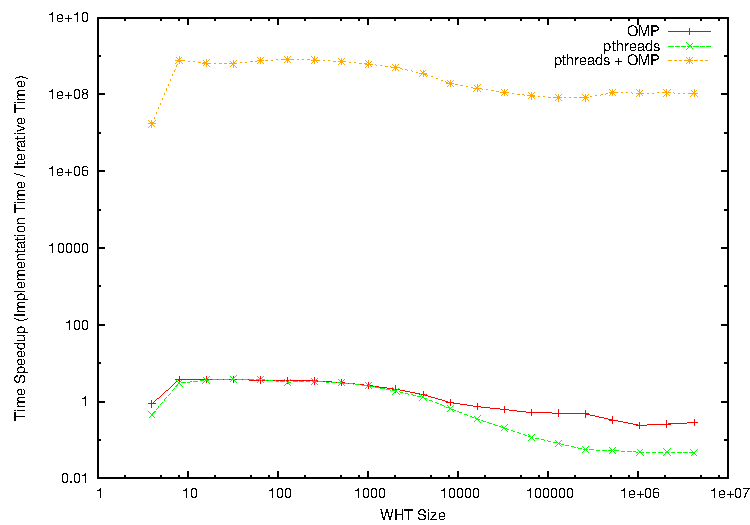
\includegraphics[width=\textwidth]{p8.pdf}
\end{document}

